\documentclass[a4paper, twoside,openright]{article}
\usepackage[T1]{fontenc} % Font encoding, T1 = it
\usepackage[utf8]{inputenc} % Input encoding - per caratteri particolari
\usepackage[english,italian]{babel} % Lingua principale italiano, con parti in inglese
\usepackage{graphicx} % Per includere immagini esterne
\usepackage[a4paper,top=3cm,bottom=3cm,left=3cm,right=3cm]{geometry} %impaginazione e margini documento
\usepackage[fontsize=13pt]{scrextend} %dimensione font
\raggedbottom % Se la pagina non è completa, lascia lo spazio alla fine
\pagestyle{headings}
\usepackage{amsmath,amsthm,amssymb,mathtools,amsfonts}
\usepackage{enumitem} 
\usepackage{filecontents}
\usepackage{chngcntr}
\usepackage{ mathrsfs }
\usepackage{xcolor}
%\usepackage[backend=bibtex]{biblatex}


%\begin{filecontents}{jobname.bib}
%	@book{coso,
%		title = {Book's title},
%		author = {Author, Some},
%		location = {The City},
%		publisher = {Publisher},
%		date = {2005},
%	}
%\end{filecontents} 


%\addbibresource{jobname.bib}


\setlength{\parindent}{0pt}
\pagenumbering{arabic}

\newcommand{\ra}{\rightarrow}
\newcommand{\Ra}{\Rightarrow}
\newcommand{\LRa}{\Leftrightarrow}
\newcommand{\R}{\mathbb{R}}
\newcommand{\N}{\mathbb{N}}
\newcommand{\Q}{\mathbb{Q}}
\newcommand{\Z}{\mathbb{Z}}
\renewcommand{\P}{\mathbb{P}}
\renewcommand{\S}{\mathbb{S}}
\newcommand{\parti}{\mathcal{P}}
\newcommand{\fa}{\forall}
\newcommand{\fo}{\forall}
\newcommand{\e}{\varepsilon}
\newcommand{\<}{\langle}
\renewcommand{\>}{\rangle}

\DeclarePairedDelimiter{\abs}{\lvert}{\rvert}
\DeclarePairedDelimiter{\norm}{\lVert}{\rVert}

\newtheorem{teo}{Teorema}[]
\newtheorem{lemma}[teo]{Lemma}
\newtheorem{defin}[teo]{Definizione}
\newtheorem{cor}[teo]{Corollario}
\newtheorem{oss}[teo]{Osservazione}
\newtheorem{es}[teo]{Esempio}
\newtheorem{prop}[teo]{Proposizione}

% Bold math in titles
\makeatletter%
\DeclareRobustCommand*{\bfseries}{%
	\not@math@alphabet\bfseries\mathbf
	\fontseries\bfdefault\selectfont
	\boldmath
}
\makeatother

\counterwithin{teo}{section}

\begin{document}

% input file frontespizio.tex
\input{frontespizio}

\tableofcontents
\clearpage

\section{Introduzione}
	 Nel $1952$ R. O. Davies dimostrò che dato un sottoinsieme misurabile dl piano $A \subset \mathbb{R}^{2}$, è possibile coprirlo con delle rette, in modo che l'insieme di punti coperto da queste rette sia abbia la stessa misura di Lebesgue di $A$.\\
	 Il nostro obiettivo è  dimostrare una generalizzazione di questo risultato per una generica misura boreliana $\sigma$-finita.
\begin{teo}
	Sia $A \subset \mathbb{R}^{2}$ misurabile e $\mu$ una misura boreliana $\sigma$-finita nel piano. Allora esiste un insieme Boreliano di rette $L$ tale che per ogni punto di $A$, l'insieme delle direzioni delle linee di $L$ contenenti il punto sia residuo e $\mu(A)=\mu(\{\bigcup \ell: \ell \in L\})$.
\end{teo} 
	In questa tesi è riportata una dimostrazione di un rafforzamento del teorema di Davies, che ne consente la generalizzazione.\\
	Il primo passo è formulare il problema in forma duale, cioè facendo corrispondere a ogni retta un punto e viceversa.\\
	Poi seguirà la dimostrazione di un lemma che attraverso una costruzione geometrica consente di affrontare parzialmente il problema.\\
	Segue la dimostrazione di Davies vera e propria e la conseguente generalizzazione.\\
	\textcolor{red}{ovviamente sistemare}


\section{Misura su insiemi di rette}

Si consideri il piano proiettivo reale $\P^2 \R$, realizzato come quoziente di $\S^2$ rispetto alla mappa $\pi$ che identifica i punti antipodali. Una misura boreliana su $\S^2$ induce tramite $\pi$ una misura di Borel su $\P^2\R$. Nel caso la misura su $\S^2$ sia misura usuale di area, chiameremo la misura immagine $\theta$.\\
Consideriamo l'insieme $M$ delle rette in $\P^2 \R$, dove ogni retta è descritta dall'equazione omogenea $ax_0+bx_1+cx_2=0$, per opportuni coefficienti $a,b,c$.\\
Possiamo identificare ogni retta con un punto di $\P^2 \R$, attraverso la bigezione $ax_0+bx_1+cx_2=0 \mapsto [a,b,c]$.\\
Data quindi una misura $\mu$ in $\P^2 \R$, si ha in modo naturale una misura boreliana su $M$, dove un boreliano di $M$ è immagine di un boreliano di $\P^2 \R$.

\begin{defin}
	Dato un insieme di rette $L \subseteq M$, diciamo che il suo duale è l'insieme di punti di $\P^2 \R$ tramite la corrispondenza descritta.\\
	Nello stesso modo, dato un insieme di punti $A \in \P^2 \R$, diciamo che il suo duale è l'insieme di rette in $M$ tramite la stessa corrispondenza.
\end{defin}	

Data una retta affine in $\R^2$, si può omogeneizzare l'equazione che la descrive e assumere che questa retta sia in in $\P^2 \R$. In questo modo, si è definita una misura anche sulle rette affini, portata dal duale. Diremo che un'insieme di rette affini è boreliano se è immagine di un boreliano tramite questa corrispondenza.\\
Alternativamente, per un insieme di rette di $\R^2$ e per $\mu$ discendente dalla misura di area su $\S^2$, si può dare una caratterizzazione degli insiemi di misura nulla come segue.

\begin{defin}
Una direzione è un punto all'infinito della chiusura proiettiva di $\R^2$. La misura sulle direzioni è l'immagine della misura di lunghezza su $S^1$, tramite il quoziente che identifica punti antipodali.\\
Dato un insieme di rette $L$ in $\R^2$ e una direzione $d$, sia $L_{d}$ l'insieme delle rette di $L$ in direzione $d$. Diciamo che $L$ contiene trascurabili rette in direzione $d$ se l'insieme di punti $\bigcup L_{d}$ ha misura di Lebesgue nulla.
\end{defin}	

\begin{lemma}
	Un insieme misurabile di rette $L$ nel piano ha misura $\theta$ nulla (secondo la misura portata dal duale) se e solo se contiene trascurabili rette in quasi ogni direzione. 
\end{lemma}

\begin{proof}
	Data una direzione $d$, $|\bigcup L_{d}|=0 \LRa$ per ogni $t_d$ retta ortogonale alla direzione $d$, $ (\bigcup L_d) \cap t_d$ ha misura lineare nulla, per il teorema di Fubini.\\
	Inoltre ogni insieme misurabile $A \subseteq \R^2$ ha misura nulla se e solo se esiste $x \in \R^2$ (equivalentemente, per ogni $x$), quasi ogni retta per $x$ interseca $A$ in insieme di misura lineare nulla. Infatti segue subito applicando il teorema di Fubini e un cambio di variabili in coordinate polari nel piano.\\
	Fissiamo $x$ punto nel duale, che corrisponde alla retta all'infinito.\\
	$|L|=0 \LRa$ per quasi ogni retta $\ell$ per $x$, $\ell \cap L$ ha misura lineare nulla.\\
	Ma l'insieme lineare $\ell \cap L$ rappresenta nel duale $L_d$, dove $d$ è la direzione (punto della retta all'infinito) che rappresenta $\ell$ nel duale. Inoltre $L_d$ è in bigezione con l'insieme lineare $(\bigcup L_d) \cap t_d$, con $t_d$ come sopra.\\
	Concludendo, $|L|=0 \LRa$ quasi per ogni direzione $d$, $(\bigcup L_d) \cap t_d$ ha misura lineare nulla $\LRa$ quasi per ogni direzione $d$, $|\bigcup L_d|=0$.
\end{proof}	

Per un insieme di rette $L$ nel piano $\R^2$, sia $L^{*}= \{\bigcup \ell | \ell \in L\}$, cioè i punti di $\R^2$ coperti da linee di $L$; per un insieme di punti $A \subseteq \R^2$, sia $A^{*}$ l'insieme delle rette per i punti di $A$.

\begin{oss}
	Sia $L$ un insieme di rette nel piano, tali che nel duale siano rappresentate da un insieme di punti appartenenti a una retta $\ell$ di equazione $ax_0+bx_1+cx_2=0$.\\
	Allora, dico che tutte le rette di $L$ passano per punto $P_{\ell}$ della chiusura proiettiva di $R^2$. Più precisamente, le coordinate proiettive di $P_{\ell}$ sono $[a,b,c]$.\\
	Infatti $z=[z_0,z_1,z_2] \in \ell \LRa az_0+bz_1+cz_2=0 \LRa [a,b,c] \in \{z_0x_0+z_1x_1+z_2x_2=0\}$.\\
	In particolare, $P_{\ell}$ è il punto che nel duale rappresenta la retta $\ell$.
\end{oss}

\begin{teo}[Versione duale del teorema di Davies]
	Data una misura boreliana $\mu$ $\sigma$-finita sull'insieme delle rette nel piano, per un insieme misurabile di rette $L$, esiste un insieme di punti $P$ tale che ogni retta di $L$ intersechi $P$ in un insieme residuo e $\mu(P^*)=\mu(L)$.
\end{teo}

\begin{proof}[Assumendo il Teorema di Davies]
	Osserviamo intanto che
	Sia $A \in \P^2\R$ il duale di $L$. A  Per il Teorema di Davies, sia $M$ insieme di rette tale che $A \subseteq M^*$ e $\mu(M^*)=\mu(A)$. Sia allora $P = \bigcup_{\ell\in M}p_\ell$. Usando l'osservazione precedente, $M^*$ è il duale di $P^*$. Segue subito che $L \subseteq P^*$ e che $|P^*|=|M^*|=|A|=|L|$.
\end{proof}

\begin{defin}
	Un insieme è residuo se il suo complementare è della prima categoria. Un insieme è della prima categoria se unione numerabile di insiemi mai densi (cioè con chiusura a parte interna vuota).
\end{defin}
Osserviamo che intersezione numerabile di aperti densi è un insieme residuo, perché il complementare è unione numerabile di insiemi mai densi.\\

Dimostreremo un rafforzamento del teorema, infatti si può scegliere $L$ in modo che per ogni punto di $A$, l'insieme delle direzioni delle rette di $L$ per il punto, sia residuo. Formulato nel caso duale, si può chiedere che fissato $L$, l'insieme di punti $A$ intersechi ogni retta in un insieme residuo.

\newpage

\section{Caso della misura di Lebesgue}

\begin{teo}
	Sia $\mu$ una misura boreliana $\sigma$-finita del piano. Allora per ogni insieme misurabile $A \subset \mathbb{R}^{2}$, esiste un insieme boreliano di rette $L$ tale che:\\
	- per ogni punto di $A$ ci sia un insieme residuo di rette di $L$, (cioè l'insieme delle direzioni delle rette di $L$ contenenti il punto sia residuo).\\
	- $\mu\left(L^{*}\right)=\mu(A)$.\\
	Nella formulazione duale, per una misura boreliana $\sigma$-finita $\mu$ sulle rette e per un insieme misurabile di rette $L$, esiste un insieme boreliano di punti $A$ tale che:\\
	- ogni retta di $L$ intersechi $A$ in un insieme residuo.\\
	- $\mu\left(A^{*}\right)=\mu(L)$.
\end{teo}

\begin{oss}
	Tale enunciato ha senso perché, come mostreremo più avanti in questa sezione, se $L$ boreliano, allora $L^{*}$ è analitico. Quindi $L^{*}$ misurabile rispetto a ogni misura boreliana nel piano. Similmente, se $A$ boreliano, $A^{*}$ è misurabile rispetto a ogni misura boreliana sullo spazio delle rette.
\end{oss}	
	
\begin{lemma}
	Nel primo enunciato del teorema, posso supporre $A$ aperto.
\end{lemma}

\begin{proof}
	Se $A$ misurabile, allora esiste $G_{\delta} = \bigcap_{n=1}^{\infty} G_{n} \supseteq A$ della stessa misura, con $G_{1} \supset G_{2} \supset \cdots$ aperti.\\
	Quindi se il teorema è verificato per gli aperti $G_{1}, G_{2}, \ldots$ e per l'insieme di rette $L_{1}, L_{2}, \ldots$, allora è anche verificato per  $A=\bigcap_{n=1}^{\infty} G_{n}$ e $L=\bigcap_{n=1}^{\infty} L_{n}$.\\
	Infatti sia $x \in G_{\delta} \subseteq G_i \quad \fa i \Ra$ l'insieme delle rette di $L_i$ per $x$ è residuo per ogni $i$. L'intersezione numerabile di tali insiemi è ancora un insieme residuo (al complementare, unione numerabile di insiemi di prima categoria è di prima categoria), in particolare è non vuoto, quindi $A \subseteq L^*$.\\
	Inoltre, $\mu(A) = \lim_n \mu(G_n) = \lim_n \mu(L_n^*) \geq \mu\left(\bigcap_{n=1}^\infty L_n^*\right) \geq \mu\left(\left(\bigcap_{n=1}^\infty L_n\right)^*\right) = \mu(L^*) \geq \mu(A)$.	
\end{proof}

Dimostriamo prima il seguente lemma, che è una versione rafforzata del teorema di Davies (nel caso della misura di Lebesgue). Si richiede non solo che $L^* \setminus A$ abbia misura nulla, ma anche che intersechi ogni retta per un dato punto in un insieme di misura lineare nulla. Ricordiamo che intersecare $quasi$ ogni retta in un insieme di misura lineare nulla è equivalente ad avere misura nulla.

\begin{lemma}
Sia $A$ aperto del piano e sia $x$ un punto che non appartiene ad $A$. Allora esiste un insieme boreliano di rette $L$ tale che:\\
- L contiene un insieme residuo di rette per ogni punto di $A$;\\
- $L^{*} \backslash A$ interseca ogni retta per $x$ in un insieme di misura di Lebesgue nulla.
\end{lemma}

Passando al duale, si ha il seguente lemma. \textcolor{orange}{non vanno fatte queste dimostrazioni vero?}

\begin{lemma}
Sia $L$ un insieme aperto di rette (cioè corrispondente nel duale a un aperto di $\P^2 \R$)e sia $X$ un retta non appartenente a $L$. Allora esiste un insieme boreliano di punti $A$ per cui:\\
- ogni retta di $L$ interseca $A$ in un insieme residuo;\\
- per ogni punto di $X$ passano trascurabili rette di $A^{*} \backslash L$.
\end{lemma}

\begin{proof} [Quest'ultimo lemma implica il precedente]
	Le condizioni del lemma si traducono in: $\fa \ell \in L, \ell^* \cap A$ è residuo; per ogni fascio di rette $M$ per un punto di $X$, $|(A^* \setminus L)\cap M|=0$. 
	
	
\end{proof}
\iffalse
($\fa y \in A, y^* \cap L$ è residuo)

($\fa \ell \ni x, |(L^* \backslash A) \cap \ell|=0$)

\fi

Possiamo assumere che $X$ sia la retta all'infinito. Allora i punti di $X$ sono direzioni di rette nel piano e possiamo formulare il precedente lemma in una versione equivalente.

\begin{lemma}
Sia $L$ un insieme aperto di rette, allora esiste un insieme di punti $A$ tale che:\\
- ogni retta di $L$ intersechi $A$ in un insieme residuo;\\
- in ogni direzione ci siano trascurabili rette di  $A^{*} \backslash L$.\\
\end{lemma}

Per dimostrarlo, usiamo il seguente lemma, la cui dimostrazione è riportata nel capitolo successivo.\\
Introduciamo anche la seguente notazione. Per un dato parallelogramma $P$ (sempre aperto e non degenere) e un intervallo di direzioni $I$, sia $A_{P, I}$ l'insieme di linee per i punti di $P$ in direzioni appartenenti a $I$.

\begin{lemma}
Per ogni parallelogramma $P$, numero positivo $\varepsilon$ e intervalli di direzioni $I, J$ tale che $\operatorname{cl}(I) \subset \operatorname{int}(J)$, esistono dei sotto parallelogrammi $P_{1}, P_{2}, \ldots$ tali che:\\
- ogni retta che interseca $P$ e la cui direzione appartiene a $I$ interseca anche uno dei parallelogrammi, cioè $\bigcup_{n} A_{P_{n}, I}=A_{P, I}$;\\
- la proiezione di $\bigcup_{n} P_{n}$ ha misura di Lebesgue minore di $\varepsilon$ in ogni direzione non appartenente a $J$.
\end{lemma}

\begin{proof}
Scegliamo $\varepsilon_{\mathbf{n}}$ positivo per ogni sequenza finita di naturali $\mathbf{n}=n_{1} n_{2} \cdots n_{k}$ tale che per ogni $k$ si abbia $\sum_{\mathbf{n}=n_{1} n_{2} \cdots n_{k}} \varepsilon_{\mathbf{n}}<1 / 2^{k}$.\\
Siano $P_{1}, P_{2}, \ldots$ parallelogrammi aperti con vertici razionali \textcolor{red}{a cosa serve?} e siano $I_{1}, I_{2}, \ldots$ intervalli aperti razionali di direzioni, tali che $A_{P_{j}, I_{j}} \subset L$ per ogni $j$, e per ogni retta $\ell \in L$, l'insieme $\left\{P_{j}: \ell \in A_{P_{j}, I_{j}}\right\}$ sia un ricoprimento di Vitali di $\ell$, cioè ogni punto di $\ell$ sia coperto da un parallelogramma arbitrariamente piccolo. l'esistenza di una configurazione di questo tipo è garantita dal fatto che $L$ sia aperto.\\
Se $P=P_{\mathbf{n}}, I=I_{\mathbf{n}}$ e $\varepsilon=\varepsilon_{\mathbf{n}}$ sono stati definiti per una sequenza finita di naturali $\mathbf{n}=n_{1} n_{2} \cdots n_{k}$, allora definiamo $P_{\mathbf{n} j}, I_{\mathbf{n} j}$ per ogni $j \in \mathbb{N}$ nel seguente modo.\\
Scegliamo dei sotto-parallelogrammi aperti razionali $P^{1}, P^{2}, \ldots$ di $P=P_{\mathbf{n}}$ e dei sotto-intervalli aperti razionali $I^{1}, I^{2}, \ldots$ di $I=I_{\mathrm{n}}$ tali che per ogni $\ell \in A_{P, I}$, l'insieme di sotto-parallelogrammi $\left\{P^{j}: \ell \in A_{P^{j}, I^{j}}\right\}$
sia un ricoprimento di Vitali del segmento $\ell \cap P$. \\
\textcolor{orange}{Posso avere $I=I_j?$}\\
Scegliamo $\varepsilon^{j}$ positivi tale che $\sum_{j} \varepsilon^{j}<\varepsilon=\varepsilon_{\mathbf{n}}$ e degli intervalli razionali di direzioni $J^{j}$ tali che $\operatorname{cl}\left(I^{j}\right) \subset \operatorname{int}\left(J^{j}\right)$ e $\sum_{j}\left|J^{j} \backslash I^{j}\right|<\varepsilon$. Si applica il Lemma 5 a tutti i parallelogrammi $P^{j}$, con intervalli $I^{j}, J^{j}$ e numeri $\varepsilon^{j}$. Otteniamo un insieme numerabile di sotto-parallelogrammi di $P$, che chiameremo $P_{\mathbf{n} 1}, P_{\mathbf{n} 2}, \ldots$. Per ogni $m$ per cui il parallelogramma $P_{\mathbf{n} m}$ è ottenuto con il Lemma 5 applicato a $P^{j}, I^{j}, J^{j}, \varepsilon^{j}$, sia $I_{\mathbf{n} m}$ l'intervallo $I^{j}$.\\
L'insieme $\left\{P^{j}: \ell \in A_{P^{j}, I^{j}}\right\}$ era un ricoprimento di Vitali di $\ell \cap P$ per ogni $\ell \in A_{P^{j}, I^{j}}$; inoltre per il primo punto del Lemma $5, \ell$ interseca uno dei sotto-parallelogrammi ottenuti applicando il lemma a $P^{j}, I^{j}, J^{j}, \varepsilon^{j}$. Quindi l'insieme $\left\{P_{\mathrm{n} m}: \ell \in A_{P_{\mathrm{nm}}, I_{\mathrm{n} m}}\right\}$
copre un sottoinsieme aperto denso del segmento $\ell \cap P$.\\
Segue che $\bigcup_{\mathbf{n}=n_{1} n_{2} \cdots n_{k}} P_{\mathbf{n}}$ interseca ogni retta $\ell \in L$ in un insieme aperto denso, quindi, per quanto osservato prima, l'insieme 
$$
A:= \bigcap_{k} \bigcup_{\mathbf{n}} P_{\mathbf{n}=n_{1} n_{2} \cdots n_{k}}
$$
interseca ogni retta $\ell \in L$ in un insieme residuo, quindi soddisfa la prima condizione del lemma 4.\\
D'altra parte, se $\ell \notin L$, o $\ell$ non interseca $P_{\mathbf{n}}$ per ogni sequenza $\mathbf{n}$, oppure esiste $\mathbf{n}$ per cui la direzione di $\ell$ non appartiene a $I_{\mathbf{n}}$.\\
Nel primo caso in particolare si ha che $\ell$ non interseca $A$.\\
Nel secondo caso, la direzione di $\ell$ non appartiene a $\bigcup_{m_{1} m_{2} \cdots m_{l}} J_{n m_{1} \cdots m_{l}}$ per $l$ abbastanza grande \textcolor{red}{perché? devo ancora usare ipotesi, immagino servano proprio qui}, quindi la proiezione di $\bigcup_{m_{1} m_{2} \cdots m_{l}} P_{\mathbf{n} m_{1} \cdots m_{l}}$ nella direzione di $\ell$ ha misura minore ho uguale a $\sum_{m_{1} m_{2} \cdots m_{l}} \varepsilon_{\mathbf{n} m_{1} \cdots m_{l}} \leq c/2^l$ per un'opportuna costante $c$. Per l'arbitrarietà di $l$, nella direzione di $\ell$ ci sono trascurabili rette che intersecano $A$. \textcolor{orange}{più precisamente dovrei aver ottenuto che in ogni direzione o ci sono solo rette che appartengono a $L$, oppure ci sono trascurabili rette. questa cosa può essere vera?}.
\textcolor{orange}{cosa sono i J con indice in basso? immagino siano definiti come gli I con indici in basso}
\end{proof}

\newpage

\section*{Generalizzazione per misure boreliane}

Nel tentativo di generalizzare il teorema per una misura boreliana $\sigma$-finita $\mu$, è necessario che, dato un insieme di rette $L$ boreliano, l'insieme di punti $L^*$ coperto da tali rette sia misurabile rispetto a $\mu$.\\
In effetti questo è vero e la dimostrazione richiede l'introduzione di alcune definizioni. 

\begin{defin}
	Sia $X$ un insieme non vuoto e sia $\mathcal{E}$ una collezione di suoi sottoinsiemi. Diciamo che $\left\{A_{n_{1}, \ldots, n_{k}}\right\}$ è uno schema di Souslin a valori in $\mathcal{E}$ se per ogni sequenza finita di naturali $\left(n_{1}, \ldots, n_{k}\right)$, si ha $A_{n_{1}, \ldots, n_{k}} \in \mathcal{E}$.\\
	L'A-operazione (o operazione di Souslin) in $\mathcal{E}$ associa a ogni schema di Souslin $\left\{A_{n_{1}, \ldots, n_{k}}\right\}$ a valori in $\mathcal{E}$ l'insieme
	$$
	A=\bigcup_{\left(n_{i}\right) \in \mathbb{N}^{\infty}} \bigcap_{k=1}^{\infty} A_{n_{1}, \ldots, n_{k}} .
	$$
	Gli insiemi in questa forma sono detti di $\mathcal{E}$-Souslin o $\mathcal{E}$-analitici. \\
	La collezione degli insiemi di questo tipo e l'insieme vuoto è indicata con $S(\mathcal{E})$.
\end{defin}	

Diciamo che uno schema di Souslin è monotono (o regolare) se $A_{n_{1}, \ldots, n_{k}, n_{k+1}} \subset A_{n_{1}, \ldots, n_{k}}$.\\
Se $\mathcal{E}$ è chiuso per intersezione finita, allora uno schema di Souslin $\left\{A_{n_{1}, \ldots, n_{k}}\right\}$ a valori in $\mathcal{E}$ può essere sostituito da uno schema monotono $\left\{A^*_{n_{1}, \ldots, n_{k}}\right\}$ avente lo stesso risultato dell'$A$-operazione. Infatti basta porre 
$$
A_{n_{1}, \ldots, n_{k}}^{*}:=A_{n_{1}} \cap A_{n_{1}, n_{2}} \cap \cdots \cap A_{n_{1}, \ldots, n_{k}} .
$$

Mostriamo intanto il seguente lemma, dove con $\left(\mathbb{N}^{\infty}\right)^{\infty}$ indichiamo lo spazio delle successioni $\eta=\left(\eta^{1}, \eta^{2}, \ldots\right)$ con $\eta^{i} \in \mathbb{N}^{\infty}$.

\begin{lemma}
	Esistono delle bigezioni
	$$	\beta: \mathbb{N} \times \mathbb{N} \rightarrow \mathbb{N} \quad \text { and } \quad \Psi: \mathbb{N}^{\infty} \times\left(\mathbb{N}^{\infty}\right)^{\infty} \rightarrow \mathbb{N}^{\infty}
	$$
	tali che per ogni $m, n \in \mathbb{N}, \sigma=\left(\sigma_{i}\right) \in \mathbb{N}^{\infty}$ e $\left(\tau^{i}\right) \in\left(\mathbb{N}^{\infty}\right)^{\infty}$, dove $\tau^{i}=\left(\tau_{j}^{i}\right) \in \mathbb{N}^{\infty}$, le collezioni $\sigma_{1}, \ldots, \sigma_{m}$ e $\tau_{1}^{m}, \ldots, \tau_{n}^{m}$ sono univocamente determinate dalle prime $\beta(m, n)$ componenti di $\Psi\left(\sigma,\left(\tau^{i}\right)\right)$.
\end{lemma}	

\begin{proof}
	Sia $\beta(m, n)=2^{m-1}(2 n-1)$. Allora $\beta$ è una bigezione da $\mathbb{N} \times \mathbb{N}$ in $\mathbb{N}$ (per unicità della fattorizzazione dei naturali). Siano $\varphi(l):=m, \psi(l):=n$, dove $\beta(m, n)=l$. Siano $\sigma=\left(\sigma_{i}\right) \in \mathbb{N}^{\infty}$ e $\left(\tau^{i}\right) \in\left(\mathbb{N}^{\infty}\right)^{\infty}$, con $\tau^{i}=\left(\tau_{j}^{i}\right) \in \mathbb{N}^{\infty}$. Poniamo
	$$
	\Psi\left(\sigma,\left(\tau^{i}\right)\right)=\left(\beta\left(\sigma_{1}, \tau_{\psi(1)}^{\varphi(1)}\right), \ldots, \beta\left(\sigma_{l}, \tau_{\psi(l)}^{\varphi(l)}\right), \ldots\right) .
	$$
	Allora per ogni $\eta=\left(\eta_{i}\right) \in \mathbb{N}^{\infty}$, l'equazione $\Psi\left(\sigma,\left(\tau^{i}\right)\right)=\eta$ ha a soluzione unica $\sigma_{i}=\varphi\left(\eta_{i}\right),  \tau_{\psi(i)}^{\varphi(i)}=\psi(\eta_i)$ da cui $\tau_{j}^{i}=\psi\left(\eta_{\beta(i, j)}\right)$. Quindi $\Psi$ è bigettiva.\\
	Poiché $m \leq \beta(m, n)$ e $\beta(m, k) \leq \beta(m, n)$ per $k \leq n$, dalla scrittura esplicita delle soluzioni $\sigma, (\tau^i)$ segue che le prime $\beta(m, n)$ componenti di $\Psi\left(\sigma,\left(\tau^{i}\right)\right)$ determinano univocamente le prime $m$ componenti di $\sigma$ e le prime $n$ componenti di $\tau^{m}$.
	
\end{proof}

Ora usiamo il precedente lemma per mostrare una proprietà generale degli insiemi di Souslin.\\

\begin{teo}
	(i) $S(S(\mathcal{E}))=S(\mathcal{E})$. In particolare, la classe $S(\mathcal{E})$ è chiusa per unioni e intersezioni numerabili.\\
	(ii) Se il complementare di ogni insieme in $\mathcal{E}$ appartiene a $S(\mathcal{E})$ (ad esempio se è unione numerabile di elementi di $\mathcal{E}$) e $\varnothing \in \mathcal{E}$, allora la $\sigma$-algebra $\sigma(\mathcal{E})$ generata da $\mathcal{E}$ è contenuta in $S(\mathcal{E}).$
\end{teo}

\begin{proof}
	Ovviamente $S(\mathcal{E}) \subset S(S(\mathcal{E}))$. Per l'altra inclusione, siano $A_{n_{1}, \ldots, n_{k}}^{\nu_{1}, \ldots, \nu_{m}} \in \mathcal{E}$ e siano
	$$ A_{n_{1}, \ldots, n_{k}}=\bigcup_{(\nu_j) \in \mathbb{N}^{\infty}} \bigcap_{m=1}^{\infty} A_{n_{1}, \ldots, n_{k}}^{\nu_{1}, \ldots, \nu_{m}} \text {. }	$$
	$$	A=\bigcup_{\left(n_{i}\right) \in \mathbb{N}^{\infty}} \bigcap_{k=1}^{\infty} A_{n_{1}, \ldots, n_{k}} \in S(S(\mathcal{E}))$$
	
	Con la stessa notazione di cui sopra, siano $\eta_{1}, \ldots, \eta_{l}$ naturali fissati. Per suriettività di $\Psi$, esistono $\sigma \in \mathbb{N}^{\infty}$ e $\tau=\left(\tau^{m}\right) \in\left(\mathbb{N}^{\infty}\right)^{\infty}$ tali che $\eta_{1}=\Psi(\sigma, \tau)_{1}, \ldots, \eta_{l}=$ $\Psi(\sigma, \tau)_{l}$. Anche se $\sigma$ e $\tau$ non sono univocamente determinate, per il lemma precedente, le collezioni $\sigma_{1}, \ldots, \sigma_{\varphi(l)}$ e $\tau_{1}^{\varphi(l)}, \ldots, \tau_{\psi(l)}^{\varphi(l)}$ lo sono. Ha senso quindi porre
	$$
	B\left(\eta_{1}, \ldots, \eta_{l}\right)=A_{\sigma_{1}, \ldots, \sigma_{\varphi(l)}}^{\tau_{1}^{\varphi(l)}, \ldots, \tau_{\psi(l)}^{\varphi(l)}} \in \mathcal{E} .
	$$
	Sia $\eta=\left(\eta_{l}\right)\in \N^{\infty}$. Mostriamo che $A=\bigcup_{\eta} \bigcap_{l=1}^{\infty} B\left(\eta_{1}, \ldots, \eta_{l}\right) \in S(\mathcal{E})$, quindi che $S(S(\mathcal{E})) \subset S(\mathcal{E})$.
	$$
	\begin{aligned}
		&\bigcup_{\eta} \bigcap_{l=1}^{\infty} B\left(\eta_{1}, \ldots, \eta_{l}\right)=\bigcup_{\sigma,\left(\tau^{m}\right)} \bigcap_{l=1}^{\infty} B\left(\Psi\left(\sigma,\left(\tau^{m}\right)\right)_{1}, \ldots, \Psi\left(\sigma,\left(\tau^{m}\right)\right)_{l}\right) \\
		&=\bigcup_{\sigma,\left(\tau^{m}\right)} \bigcap_{l=1}^{\infty} A_{\sigma_{1}, \ldots, \sigma_{\varphi(l)}}^{\tau_{1}^{\varphi(l)}, \ldots, \tau_{\psi(l)}^{\varphi(l)}}=\bigcup_{\sigma,\left(\tau^{m}\right)} \bigcap_{m, n=1}^{\infty} A_{\sigma_{1}, \ldots, \sigma_{m}}^{\tau_{1}^{m}, \ldots, \tau_{n}^{m}} \\
		&=\bigcup_{\sigma} \bigcup_{\left(\tau^{m}\right)} \bigcap_{m=1}^{\infty} \bigcap_{n=1}^{\infty} A_{\sigma_{1}, \ldots, \sigma_{m}}^{\tau_{1}^{m}, \ldots, \tau_{n}^{m}}=\bigcup_{\sigma} \bigcap_{m=1}^{\infty} \bigcup_{\tau^{m}} \bigcap_{n=1}^{\infty} A_{\sigma_{1}, \ldots, \sigma_{m}}^{\tau_{1}^{m}, \ldots, \tau_{n}^{m}} \\
		&=\bigcup_{\sigma} \bigcap_{m=1}^{\infty} A_{\sigma_{1}, \ldots, \sigma_{m}}=A
	\end{aligned}
	$$
	Per concludere che $S(\mathcal{E})$ chiuso per intersezioni e unioni numerabili, consideriamo degli insiemi $B_1, B_2...$ in $S(\mathcal{E})$. Allora ponendo $A_{n_1,...,n_k}=B_{n_1}$ se $n_1=...=n_k$ e vuoto altrimenti, l'$A$-operazione dà l'unione numerabile dei $B_n$.\\
	Similmente, ponendo $A_{1,2,3,...,k}=B_{k}$ e vuoto altrimenti,  l'$A$-operazione dà l'intersezione numerabile dei $B_n$.\\
	(ii) Sia
	$$
	\mathcal{F}=\{B \in S(\mathcal{E}): \quad X \backslash B \in S(\mathcal{E})\} .
	$$
	Mostriamo che $\mathcal{F}$ è una $\sigma$-algebra. Per costruzione, $\mathcal{F}$ è chiusa per complementare. Siano $B_{n} \in \mathcal{F}$, allora $\bigcap_{n=1}^{\infty} B_{n} \in S(\mathcal{E})$ per l'enunciato (i). Similmente, $X \backslash \bigcap_{n=1}^{\infty} B_{n}=\bigcup_{n=1}^{\infty}\left(X \backslash B_{n}\right) \in S(\mathcal{E})$, da cui $\mathcal{F}$ chiusa per intersezione. Inoltre per l'ipotesi, $\varnothing \in \mathcal{F}$. Quindi $\mathcal{F}$ è una $\sigma$-algebra. Per ipotesi $\mathcal{E} \subset \mathcal{F}$, da cui $\sigma(\mathcal{E}) \subset \mathcal{F} \subset S(\mathcal{E})$.\\
\end{proof}

\begin{defin}
	Data una funzione non negativa $\mu$ definita su una classe $\mathcal{A}$ di sottoinsiemi di uno spazio $X$ che contiene $X$ stesso, la misura esterna è una funzione non negativa sui sottoinsiemi di $X$, definita come segue
	$$ \mu^*(A) = \inf \{ \sum_{n=1}^{\infty} \mu (A_n) | A_n \in \mathcal{A}, A \subseteq \bigcup_{n=1}^{\infty} A_n \} $$
	Un insieme $A$ è $\mu-misurabile$ se per ogni $\varepsilon > 0$ esiste $A_{\varepsilon} \in \mathcal{A}$ tale che $\mu^*(A \ \Delta \ A_{\varepsilon}) < \varepsilon$.
\end{defin}	


\begin{teo}
	Sia $\mu$ una misura finita su una $\sigma$-algebra $\mathcal{M}$. Allora la classe $\mathcal{M}_{\mu}$ di tutti gli insiemi $\mu$-misurabili è chiuso rispetto all'A-operazione. Inoltre, data una famiglia di insiemi $\mathcal{E} \subset \mathcal{M}$ chiusa rispetto a unioni finite e intersezioni numerabili vale
	$$
	\mu^{*}(A)=\sup \{\mu(E): E \subset A, E \in \mathcal{E}\}
	$$
	per ogni $\mathcal{E}$-insieme di Souslin $A$. In particolare, ogni $\mathcal{E}$-insieme di Souslin è $\mu$-misurabile.
\end{teo}

\begin{proof}
	Il primo enunciato segue applicando il secondo alla famiglia $\mathcal{E}=\mathcal{M}_{\mu}$, perché $\mathcal{M}_{\mu}$ soddisfa le ipotesi del secondo enunciato, quindi si ha $S(\mathcal{M}_{\mu}) \subseteq \mathcal{M}_{\mu} \subseteq S(\mathcal{M}_{\mu})$.\\
	Per mostrare il secondo enunciato, sia $A$ costruito con l'A-operazione a partire da uno schema di Souslin di insiemi $E_{n_{1}, \ldots, n_{k}} \in \mathcal{E}$. Siccome $\mathcal{E}$ chiuso per intersezione finita, posso supporre che sia uno schema monotono.\\
	Sia $\varepsilon>0$. Per ogni collezione $m_{1}, \ldots, m_{k}$ di numeri naturali, indichiamo con $D_{m_{1}, \ldots, m_{k}}$ l'unione di $E_{n_{1}, \ldots, n_{k}}$ per $n_{1} \leq m_{1}, \ldots, n_{k} \leq m_{k}$. Poiché lo schema di Souslin è decrescente, anche la famiglia $D_{m_1,...,m_k}$ è decrescente in $k$.\\
	Sia
	$$
	M_{m_{1}, \ldots, m_{k}}:=\bigcup_{\left(n_{i}\right) \in \mathbb{N}^{\infty}, n_{1} \leq m_{1}, \ldots, n_{k} \leq m_{k}}^{\infty} \bigcap_{j=1}^{\infty} E_{n_{1}, \ldots, n_{j}} .
	$$
	Per $k, m_1,...,m_k \rightarrow \infty$, gli insiemi $M_{m_1,...,m_k}$ tendono crescendo ad $A$ e, fissati $m_{1}, \ldots, m_{k}$ gli insiemi $M_{m_{1}, \ldots, m_{k}, m}$  tendono crescendo a $M_{m_{1}, \ldots, m_{k}}$ per $m \rightarrow \infty$.\\
	Ricordando che la misura esterna passa al limite per unioni numerabili monotone, esiste un numero $m_{1}$ con $\mu^{*}\left(M_{m_{1}}\right)>\mu^{*}(A)-\varepsilon 2^{-1}$. Nello stesso modo esiste un numero $m_{2}$ con $\mu^{*}\left(M_{m_{1}, m_{2}}\right)>\mu^{*}\left(M_{m_{1}}\right)-\varepsilon 2^{-2}$. Induttivamente, otteniamo una successione di naturali $m_{k}$ tali che
	$$
	\mu^{*}\left(M_{m_{1}, m_{2}, \ldots, m_{k}}\right)>\mu^{*}\left(M_{m_{1}, m_{2}, \ldots, m_{k-1}}\right)-\varepsilon 2^{-k} .
	$$
	Quindi per ogni $k$ si ha
	$$
	\mu^{*}\left(M_{m_{1}, m_{2}, \ldots, m_{k}}\right)>\mu^{*}(A)-\varepsilon .
	$$
	Poiché $\mathcal{E}$ chiuso per unioni finite, $D_{m_{1}, \ldots, m_{k}} \in \mathcal{E}$; poiché $\mathcal{E}$ chiuso per intersezioni numerabili, $E:=\bigcap_{k=1}^{\infty} D_{m_{1}, \ldots, m_{k}} \in \mathcal{E}$. Siccome $M_{m_{1}, \ldots, m_{k}} \subset D_{m_{1}, \ldots, m_{k}}$, usando la precedente stima, $\mu^{*}\left(D_{m_{1}, m_{2}, \ldots, m_{k}}\right)>\mu^{*}(A)-\varepsilon$. Quindi $\mu(E) \geq \mu^{*}(A)-\varepsilon$, perché gli insiemi $D_{m_{1}, m_{2}, \ldots, m_{k}}$ decrescono a $E$.\\
	Mostriamo infine che $E \subset A$. Sia $x \in E$, cioé per ogni $k$ si ha $x \in D_{m_{1}, \ldots, m_{k}}$. Quindi $x \in E_{n_{1}, \ldots, n_{k}}$ per una collezione $n_{1}, \ldots, n_{k}$ tale che $n_{1} \leq m_{1}, \ldots, n_{k} \leq m_{k}$.\\
	Chiameremo queste collezioni ammissibili e costruiremo una successione infinita $n_{1}, n_{2}, \ldots$ con intervalli iniziali $n_{1}, \ldots, n_{k}$ ammissibili.	In tal caso, si avrà $x \in \bigcap_{k=1}^{\infty} E_{n_{1}, \ldots, n_{k}} \subset A$.\\
	Per costruirla, osserviamo che, per ogni $k>1$, abbiamo collezioni ammissibili di $k$ numeri. Diciamo che una collezione $n_{1}, \ldots, n_{k}$ è estendibile se, per ogni $l \geq k$, esiste una collezione ammissibile $p_{1}, \ldots, p_{l}$ tale che $p_1=n_1,...,p_k=n_k$.\\
	Osserviamo che ogni intervallo iniziale $n_{1}, \ldots, n_{k}$ in una collezione ammissibile prova $n_{1}, \ldots, n_{k}, \ldots, n_{l}$ è ammissibile per monotonia (cioé $E_{n_{1}, \ldots, n_{l}} \subset E_{n_{1}, \ldots, n_{k}}$).\\
	Concludiamo che esiste almeno una collezione estendibile di lunghezza $1$. Infatti, supponendo il contrario, si ha che per ogni $n \leq m_{1}$ esiste una lunghezza massima $l(n)$ delle collezioni ammissibili con il numero $n$ in prima posizione. Infatti per un certo $n$ se tale massimo non esistesse, per l'osservazione precedente, la collezione $n$ sarebbe estendibile. Ora, i finiti valori di $l(n)$, sono uniformemente limitati, da cui le collezioni ammissibili hanno lunghezza limitata,che è assurdo.\\
	Con lo stesso procedimento, la collezione estendibile $n_{1}$ è contenuta in un'altra $n_{1}, n_{2}$ estendibile. Induttivamente si ottiene una successione che per costruzione soddisfa la tesi.\\
	Infine, come conseguenza del secondo enunciato, dato $A \in S(\mathcal{E})$, per ogni $\varepsilon >0$ esiste $E \in \mathcal{E}$ tale che $\mu^*(A \setminus E) < \varepsilon$, quindi $A$ misurabile.

\end{proof}

Scegliendo come $\mathcal{E}=\mathcal{K}$, l'insieme dei compatti nello spazio delle linee (cioè compatti di $\P^2 \R$), le ipotesi del teorema ... sono verificate: infatti ogni aperto di $\P^2 \R$ è unione numerabile di compatti e $\varnothing \in \mathcal{K}$. Quindi $\sigma(\mathcal{K})=\mathcal{B} \subseteq S(\mathcal{K})$ dove con ${\cal B}$ si indicano i boreliani di $\P^2R$.\\

Tornando al problema specifico del teorema di Davies, consideriamo un insieme boreliano di rette affini $L$. Per quanto appena dimostrato e poiché $\mathcal{K}$ chiuso per intersezione finita, esiste uno schema di Souslin monotono di insiemi compatti di linee che rappresenta $L$ tramite l'$A$-operazione, cioè
$$L=\bigcup_{{\bf n}\in{\bf N}^\infty}\bigcap_{k=1}^\infty K_{n_1,\ldots,n_k}$$
con $K_{n_1,\ldots,n_k}\in {\cal K}$.\\
Siccome la mappa $L \mapsto L^*$ commuta con l'unione arbitraria, vale
$$L^*=\bigcup_{{\bf n}\in{\bf N}^\infty}\biggl(\bigcap_{k=1}^\infty K_{n_1,\ldots,n_k}\biggr)^*.$$
Mostriamo che tale mappa commuta anche con intersezioni decrescenti di compatti, cioè
$$\biggl(\bigcap_{k=1}^\infty K_{n_1,\ldots,n_k}\biggr)^*=\bigcap_{k=1}^\infty K^*_{n_1,\ldots,n_k}\leqno $$
L'inclusione $\subseteq$ è sempre vera. Viceversa, sia $x$ per cui esistono linee ${\ell_k}$ per cui $x\in \ell_k\in K^*_{n_1,\ldots,n_k}$ per ogni $k$. Per compattezza esiste una linea $\ell$, limite di una sottosuccessione delle $\ell_k$ che per monotonia deve appartenere a tutti i $K^*_{n_1,\ldots,n_k}$. Inoltre poiché il passaggio per $x$ è una condizione chiusa, $\ell$ contiene ancora $x$.\\
Se mostriamo che i $K^*_{n_1,\ldots,n_k}$ sono analitici, poiché l'$A$-operazione mantiene l'analiticità, anche $L^*$ analitico.\\
Siccome $L$ insieme di linee affini e lo schema di Souslin è monotono, posso supporre che ogni $K_{n_1,...,n_k}$ non contenga la retta all'infinito.\\
Sia quindi $K$ insieme di linee affini compatto. L'insieme $K_0$ delle linee in $K$ che sono verticali è un compatto. Quindi i punti di $K_0^*$ appartengono al prodotto di un compatto per $\R$, che è analitico perché chiuso.\\
L'insieme $K_1$ delle rette in $K$ non verticali è omeomorfo a un chiuso di $\R^2$ tramite la carta $[a,b,c] \mapsto (a/c,b/c)$ (ricordiamo che $[a,b,c]$ identifica la retta di equazione $ax_0+bx_1+cx_2=0$). Un insieme di linee parametrizzate da un rettangolo di $\R^2$, è l'insieme di linee passanti per un intervallo dell'asse $y$ aventi direzioni in un certo intervallo. Allora l'insieme di punti coperto da tali linee è un boreliano, quindi analitico.\\
Ora, dato un chiuso $C$ di $\R^2$, esistono rettangoli aperti per cui $\bigcup_n A_n = C^c$. Siano $R_m$ rettangoli chiusi tali che $\bigcup_m R_m = \R^2$. Allora $\bigcap_n(A_n^c \cap R_m)=C \cap R_m$ è intersezione numerabile di compatti, ciascuno dei quali è unione finita di rettangoli. Inoltre $C=\bigcup_m(R_m \cap C)$. Quindi utilizzando unioni numerabili e intersezioni numerabili di compatti, otteniamo che la tesi è vera per ogni chiuso $C$.\\ 

Ora possiamo dimostrare il teorema 1
\begin{proof}
Siano $K_{1} \subset K_{2} \subset \cdots$ compatti di $\mathbb{R}^{2} \backslash A$ tali che $\mu\left(\left(\mathbb{R}^{2} \backslash A\right) \backslash \bigcup_{n} K_{n}\right)=0$ e sia $\mu_{n}$ la restrizione di $\mu$ all'insieme $K_{n}$. Basta mostrare che esiste un insieme di rette $L_{n}$ tali che la tesi valga per $L_{n}$ e $\mu_{n}$. Infatti, con una dimostrazione simile a quella del lemma ..., la tesi vale per $\bigcap_{n=1}^{\infty} L_{n}$ e $\mu$. Quindi possiamo assumere che $\mu$ abbia supporto compatto $K$ disgiunto da $A$.\\
Scegliamo numerabili palle aperte $B\left(x_{n}, r_{n}\right)$ tali che
$$
A \subset \bigcup_{n}\left(B\left(x_{n}, r_{n}\right) \backslash\left\{x_{n}\right\}\right)
$$
e $B\left(x_{n}, 2 r_{n}\right) \cap K=\varnothing$ per ogni $n$.\\
Basta mostrare che esiste un insieme di rette $L_{n}$ tale che la tesi valga per $B\left(x_{n}, r_{n}\right) \backslash\left\{x_{n}\right\}$ e $\mu$.\\
Infatti $\bigcup_n L_n$ copre $A$; inoltre per ogni $n$, $\mu(L_n^* \backslash B(x_n,r_n))=\mu(L_n^*)=0$ perché il supporto di $\mu$ è $K$ disgiunto da $B(x_n,r_n))$, quindi $\mu((\bigcup_nL_n)^*) \leq \mu(\bigcup_n L_n^*)=0$. Quindi possiamo assumere che $A=B(x, r) \backslash\{x\}$ e $B(x, 2 r)$ sia disgiunta da $K$.\\
Per brevità, assumiamo che $A=B(0,1) \backslash\{0\}$ e $B(0,2) \cap K=\varnothing$. Applichiamo il lemma 2 ad $A$ e $x=0$, e sia $M$ l'insieme di rette così ottenuto.\\
Sia $M^{* *}=M^{*} \backslash B(0,1)$. Consideriamo lo spazio
$$
\left(\mathbb{R}^{2}, \mu\right) \times(\mathbb{R}, \lambda),
$$
dove $\lambda$ è la misura di Lebesgue sulla retta e consideriamo il sottoinsieme
$$
\left\{(x, t) \in \mathbb{R}^{2} \times \mathbb{R}: t x \in M^{* *}\right\} .
$$
Poiché $M$ soddisfa la seconda condizione del lemma 2, $M^{**}$ interseca ogni retta per l'origine in un insieme di misura di Lebesgue nulla, cioè per ogni $x \neq 0$ vale $\lambda(\{t: tx \in M^{**}\})=0$ (tutte le sezioni verticali di questo sottoinsieme hanno misura di Lebesgue nulla). Quindi quasi ogni sezione orizzontale ha misura nulla e possiamo scegliere un numero $u$ tale che $1 / 2<u<1$ e $\mu\left(\left\{x: u x \in M^{* *}\right\}\right)=0$, e porre $t=1 / u$. Quindi $1<t<2$ e $\mu\left(t M^{* *}\right)=0$. Affermiamo che $t M$ soddisfa la tesi.\\
Siccome $M$ contiene residue rette per ogni punto di $B(0,1) \backslash\{0\}$, $t M$ contiene residue rette per i punti di $t B(0,1) \backslash\{0\}$, ma $t B(0,1) \backslash\{0\} \supset B(0,1) \backslash\{0\}=A$ quindi è vera la prima affermazione.\\
D'altra parte, siccome $B(0,2) \cap K=\varnothing$ e $t<2$, si ha
$$
\mu\left(t M^{*}\right)=\mu\left(t M^{*} \cap K\right)=\mu\left(t M^{*} \backslash B(0, t)\right)
$$
Inoltre
$$
t M^{*} \backslash B(0, t)=t\left(M^{*} \backslash B(0,1)\right)=t M^{* *}
$$
Siccome $\mu\left(t M^{* *}\right)=0$, anche $\mu (tM^*)= 0= \mu(A)$.

\end{proof}

\newpage

\section{Costruzione per parallelogrammi}

Per dimostrare il lemma 5, introduciamo una costruzione geometrica (detta "venetian blind"), che a un parallelogramma $P_1$, associa dei sotto-parallelogrammi con le proprietà seguenti: la misura della loro proiezione in alcune direzioni sia piccola, mentre in altre direzioni sia la stessa della proiezione di $P$.\\
Consideriamo il parallelogramma non degenere $P=A_{1} A_{2} A_{3} A_{4}$, con punti medi dei lati $B_{1}, B_{2}, B_{3}, B_{4}$, come in figura 1. Sia $C$ il centro del parallelogramma. Il primo passo consiste nel scegliere i due sotto-parallelogrammi $A_{1} C B_{3} B_{4}$ e $B_{1} B_{2} A_{3} C$ (evidenziati in figura).

\begin{center}
	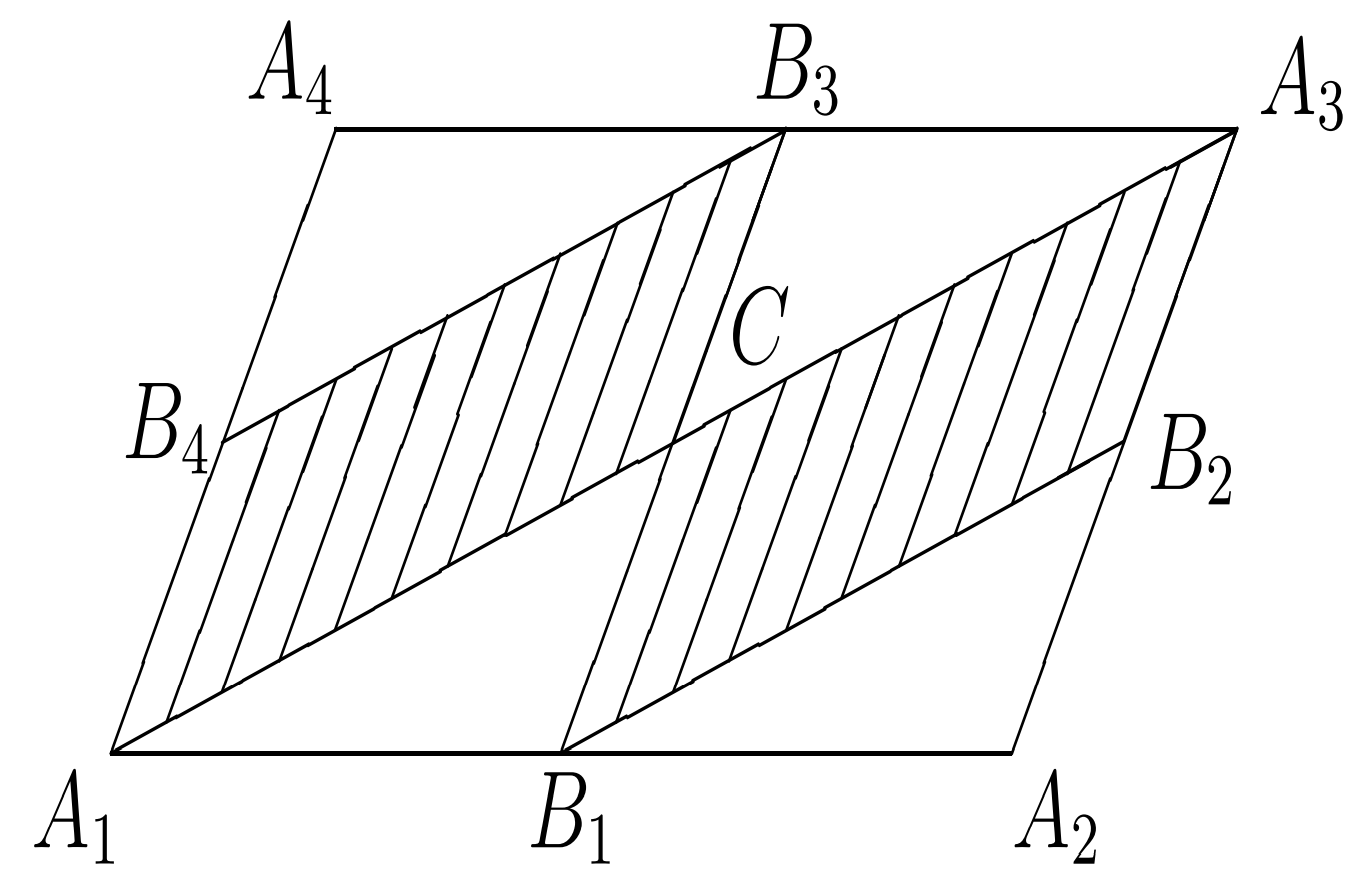
\includegraphics[width=0.5\columnwidth]{passo1.png}
\end{center}

Ora ripetiamo il procedimento per ciascuno dei nuovi parallelogrammi. Iterando per un numero finito di passi, si ottengono un numero finito di sotto-parallelogrammi di $P$. Nella figura 2 sono mostrati i primi tre passi e sono evidenziati gli otto parallelogrammi ottenuti.\\

\begin{center}
	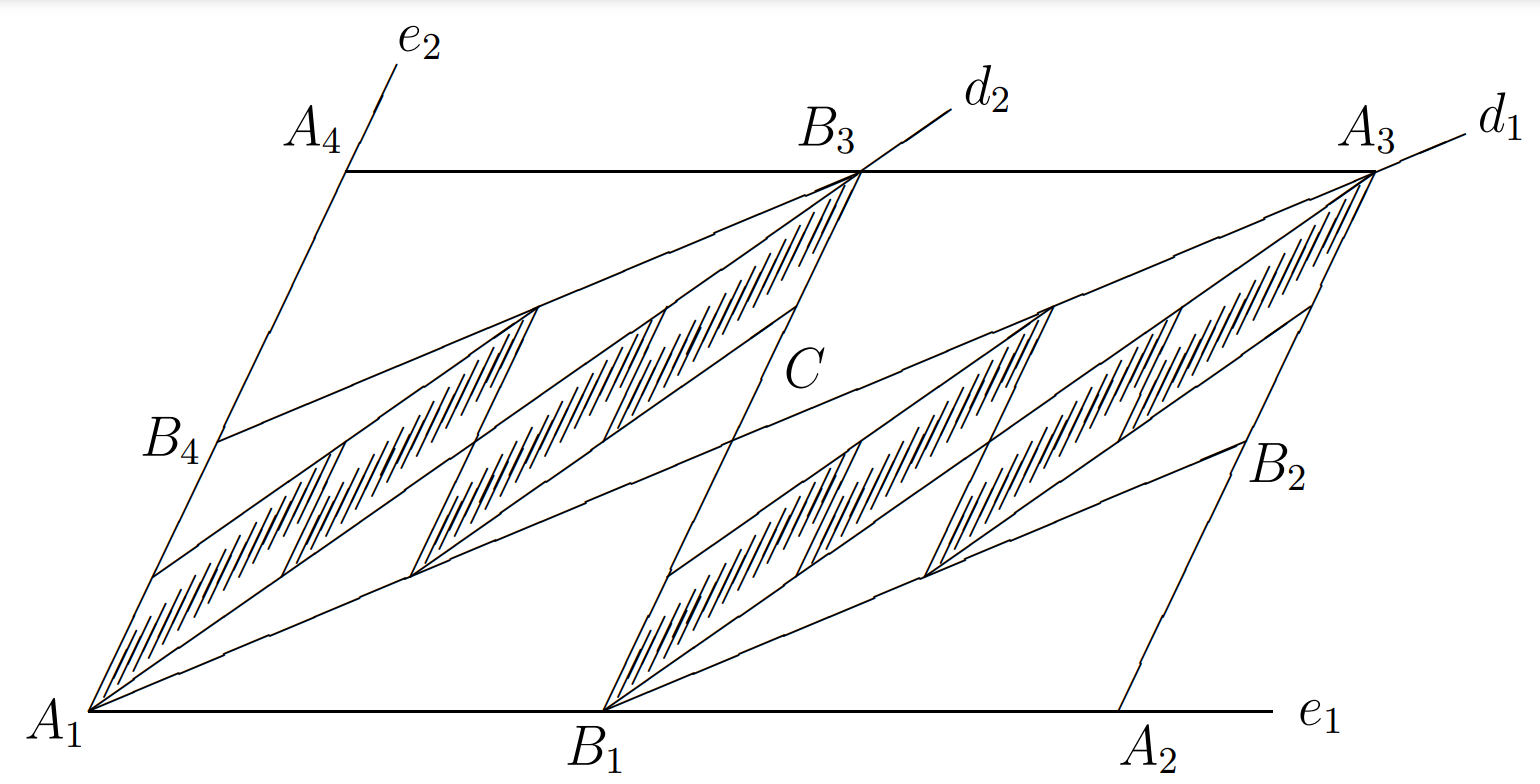
\includegraphics[width=0.7\columnwidth]{passi123.png}
\end{center}

Siano $e_{1}, e_{2}$ le direzioni dei lati di $P$ e siano $d_{1}, d_{2}, \ldots$ le direzioni delle diagonali $A_{1} A_{3}, A_{1} B_{3},...$. Sia ha che $d_{n} \rightarrow e_{2}$.\\
Come illustrato nella figura seguente, definiamo dei sotto insiemi di direzioni come segue. Sia $D_1$ l'insieme delle direzioni delle rette per $A_{4}$ che intersecano $A_{1} A_{3}$; $D_2$ l'insieme di direzioni tra $e_{1}$ e $d_{1}$; $D_3$ l'insieme delle direzioni tra $d_{1}$ e $d_{2}$, ...\\
Notiamo che data una direzione diversa da quella verticale, esiste un $n$ abbastanza grande per cui tale direzione appartenga a $D_n$.

\begin{center}
	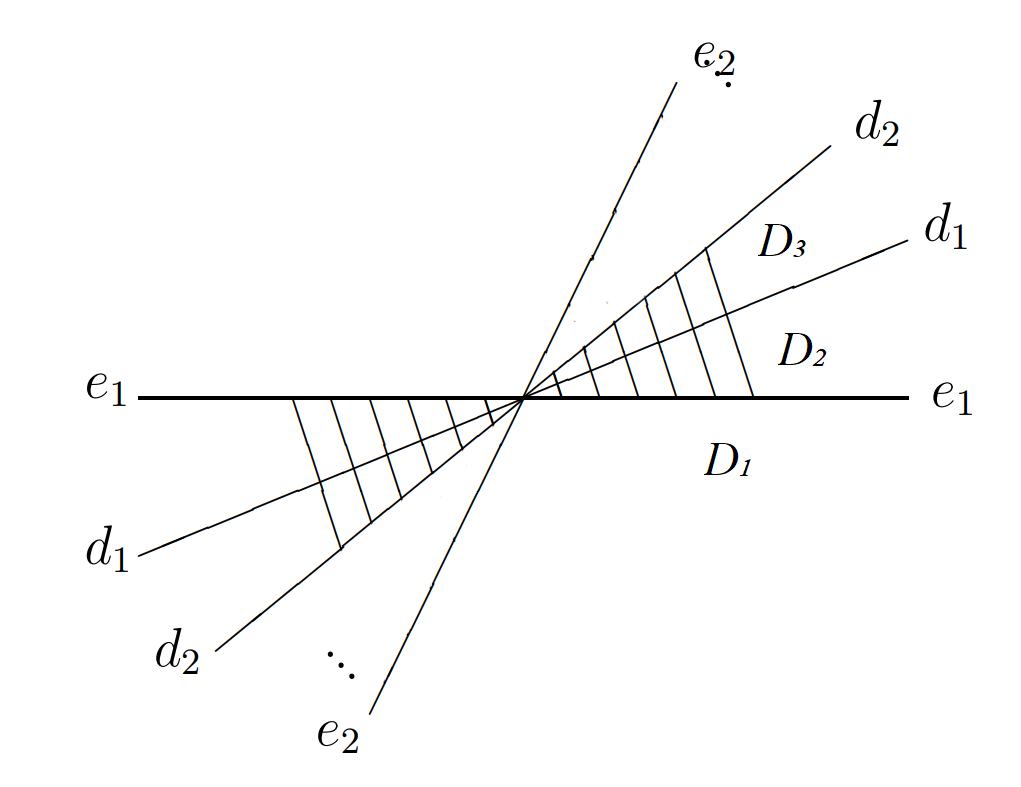
\includegraphics[width=0.6\columnwidth]{direzioni.png}
\end{center}

Ogni retta in direzione appartenente a $D_1$ che interseca $P$ interseca anche la diagonale $A_{1} A_{3}$, quindi uno dei parallelogrammi $A_{1} C B_{3} B_{4}$ e $B_{1} B_{2} A_{3} C$.\\
Inoltre, si vede facilmente che la misura delle proiezioni di ciascuno di questi parallelogrammi sulla retta $A_{1} A_{4}$ è al più $\left|A_{1} A_{4}\right|$ in ogni direzione in $D_2$. Quindi la misura della proiezione dell'unione dei parallelogrammi è al più $2 \cdot\left|A_{1} A_{4}\right|$.\\
Nello stesso modo, ogni retta in direzione in $D_1$ o $D_2$ che interseca $A_{1} C B_{3} B_{4}$ o $B_{1} B_{2} A_{3} C$ interseca uno dei 4 parallelogrammi del secondo passo. Inoltre la misura della proiezione dell'unione dei 4 parallelogrammi sulla retta $A_{1} A_{4}$ nelle direzioni in $D_3$ è al più $4 \cdot\left|A_{1} B_{4}\right|=2 \cdot\left|A_{1} A_{4}\right|$. In realtà, quest'ultima proprietà vale anche per le direzioni in $D_2$.\\

Induttivamente, all'$n$-esimo passo, le rette in direzioni appartenenti a $\bigcup_{i=1}^n D_i$ intersecano l'unione dei parallelogrammi costruiti all'$n$-esimo passo, se intersecano uno dei parallelogrammi del passo $n-1$. In particolare una retta in direzione in $D_1$ che interseca $P$, interseca uno dei parallelogrammi dell'$n$-esimo passo.\\
Inoltre la misura della proiezione dell'unione dei parallelogrammi dell'$n$-esimo passo sulla retta $A_{1} A_{4}$ è al più $2 \cdot\left|A_{1} A_{4}\right|$ in ogni direzione in $\bigcup_{i=2}^{n+1}$.\\

\begin{lemma}
	Sia $I=\left\{I^{1}, I^{2}, \ldots, I^{m}\right\}$ un insieme finito di intervalli due a due disgiunti di direzioni e sia $J=\left\{J^{1}, J^{2}, \ldots, J^{m}\right\}$ un insieme di sotto intervalli stretti (cioè, $\operatorname{cl}\left(J^{j}\right) \subset \operatorname{int} I^{j}$ per ogni $j$). Allora per ogni parallelogramma $T$ e $\varepsilon>0$ esistono dei parallelogrammi disgiunti $T_{1}, T_{2}, \ldots \subset T$ tali che:\\
	- per ogni $e \in \cup J$ la proiezione di $U$ in direzione $e$ abbia misura minore di $\varepsilon$;\\
	- per ogni retta $l$ in direzione $e \notin \cup I$, se $l$ interseca $T$ allora $l$ interseca anche $U$.	
\end{lemma}	

\begin{proof}
	Assumiamo $m=1$, con intervalli $J \subseteq I$. Sia $T$ parallelogramma non degenere, allora scegliamo un intervallo $(a, b)$ tale che $\operatorname{cl}(J) \subsetneq(a, b) \subset[a, b] \subsetneq \operatorname{int}(I)$.\\
	Allora possiamo scegliere dei vertici di $T$ e dei parallelogrammi due a due disgiunti in $T$ e tali che:\\
	- le direzioni dei lati di tutti i parallelogrammi siano $a$ e $b$;\\
	- ogni retta in direzione in $I^c$ che interseca $T$ interseca anche uno dei sotto-parallelogrammi;\\
	- la somma dei lati in direzione $a$ sia minore di $\frac{1}{2} \varepsilon$, dove $\varepsilon$ è un numero positivo fissato.\\
	Detti questi $\{T_n\}_{n \in \N}$, applichiamo la procedura esposta sopra ad ogni $T_i$, in modo che il lato $A_1A_4$ sia in direzione $a$, con riferimento alla notazione precedente.\\
	Il numero di passi necessario è indipendente dal $T_i$ scelto ed è dato dalla seguente osservazione: poiché $\operatorname{cl}(J) \subsetneq(a, b)$, esiste $\rho >0$ tale che $J \subset (a+\rho,b)$. Quindi esiste un certo $n$ per cui $J \subseteq \bigcup_{i=2}^{n+1}D_i$.\\
	Con questa procedura si ottiene un nuovo sistema di sotto-parallelogrammi e la misura della proiezione (non ortogonale) dell'unione di questi sulla linea di direzione $a$ è minore di $2 \cdot \frac{1}{2} \varepsilon=\varepsilon$ in ogni direzione in $J$. Quindi, la misura della proiezione ortogonale in ogni direzione in $J$ è minore di $\varepsilon$.\\
	Infine siccome $D_1 =(a,b)^c$ e $(a,b) \subseteq I$, allora $I^c \subseteq D_1$. Quindi ogni retta in direzione di $I^c$ che interseca uno dei $T_i$, interseca anche uno dei finiti sotto-parallelogrammi di $T_i$ definiti all'$n$-esimo passo.\\
\end{proof}

%\printbibliography

\end{document}